\documentclass[tikz]{standalone}
\usetikzlibrary{calc, positioning, arrows, arrows.meta}
\usetikzlibrary{intersections}
\begin{document}
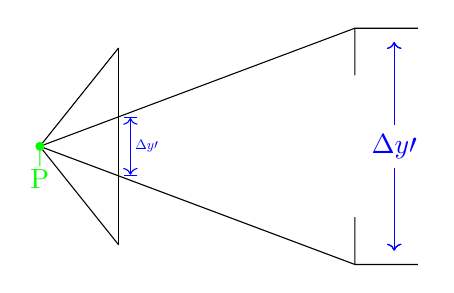
\begin{tikzpicture}

  \coordinate (pose-gt)    at (-1,  0);
  \coordinate (near-left)  at (3,  1.5);
  \coordinate (near-right) at (3, -1.5);

  \draw ($(near-left)!0.2!(near-right)$) to (near-left) to ($(near-left) + (0.8, 0)$);

  \draw ($(near-right)!0.2!(near-left)$) to (near-right) to ($(near-right) + (0.8, 0)$);

  \draw[name path=ray-left]  (pose-gt) to ($(pose-gt)!1.0!(near-left)$);
  \draw[name path=ray-right] (pose-gt) to ($(pose-gt)!1.0!(near-right)$);

  % draw lens
  \coordinate (lens-left) at ($(pose-gt)  + (1.0,  1.25)$);
  \coordinate (lens-right) at ($(pose-gt) + (1.0, -1.25)$);
  \draw (pose-gt) to (lens-left);
  \draw (pose-gt) to (lens-right);
  \draw[name path=lens-front] (lens-left) to (lens-right);

  % lens ray interections
  \fill[name intersections={of=ray-left and lens-front, name=i}] coordinate (ray-left-inter) at (i-1);
  \fill[name intersections={of=ray-right and lens-front, name=i}] coordinate (ray-right-inter) at (i-1);

  \draw[|<->|, blue] ($(ray-left-inter) + (0.15, 0)$) to node[fill=white, opacity=0.5, text opacity=1, scale=0.5, right] {$\Delta y\prime$} ($(ray-right-inter) + (0.15, 0)$);


  \draw[<->, shorten <=5, shorten >=5, blue] ($(near-left) + (0.5, 0)$) to node[fill=white] {$\Delta y\prime$} ($(near-right) + (0.5, 0)$);

  \draw[<->, shorten <=5, shorten >=5, blue] ($(near-left) + (0.5, 0)$) to node[fill=white] {$\Delta y\prime$} ($(near-right) + (0.5, 0)$);

  \draw[green, fill] (pose-gt) circle[radius=0.05] to ++(0., -0.25) node[anchor=north, inner sep=1.0]{P};



\end{tikzpicture}

\end{document}
